% --------------------------------------------------------------
% This is all preamble stuff that you don't have to worry about.
% Head down to where it says "Start here"
% --------------------------------------------------------------
 
\documentclass[10pt]{article}

 \usepackage{tikz}
\usepackage[margin=1in]{geometry} 
\usepackage{amsmath,amsthm,amssymb}
 
\newcommand{\N}{\mathbb{N}}
\newcommand{\Z}{\mathbb{Z}}
 
\newenvironment{theorem}[2][Theorem]{\begin{trivlist}
\item[\hskip \labelsep {\bfseries #1}\hskip \labelsep {\bfseries #2.}]}{\end{trivlist}}
\newenvironment{lemma}[2][Lemma]{\begin{trivlist}
\item[\hskip \labelsep {\bfseries #1}\hskip \labelsep {\bfseries #2.}]}{\end{trivlist}}
\newenvironment{exercise}[2][Exercise]{\begin{trivlist}
\item[\hskip \labelsep {\bfseries #1}\hskip \labelsep {\bfseries #2.}]}{\end{trivlist}}
\newenvironment{reflection}[2][Reflection]{\begin{trivlist}
\item[\hskip \labelsep {\bfseries #1}\hskip \labelsep {\bfseries #2.}]}{\end{trivlist}}
\newenvironment{proposition}[2][Proposition]{\begin{trivlist}
\item[\hskip \labelsep {\bfseries #1}\hskip \labelsep {\bfseries #2.}]}{\end{trivlist}}
\newenvironment{corollary}[2][Corollary]{\begin{trivlist}
\item[\hskip \labelsep {\bfseries #1}\hskip \labelsep {\bfseries #2.}]}{\end{trivlist}}
\newenvironment{solution}[2][Solution]{\begin{trivlist}
\item[\hskip \labelsep {\bfseries #1}\hskip \labelsep {\bfseries #2.}]}{\end{trivlist}}

\theoremstyle{definition}
\newtheorem*{defn*}{Definition}
\newtheorem{conj}{Conjecture}[section]
\newtheorem{exmp}{Example}[section]
\newtheorem{bas}{Basis}[section]

 
\begin{document}
 
% --------------------------------------------------------------
%                         Start here
% --------------------------------------------------------------
 
%\renewcommand{\qedsymbol}{\filledbox}
 
\title{CS310: Homework 3}%replace X with the appropriate number
\author{Scott Fenton\\ %replace with your name
} %if necessary, replace with your course title
 
\maketitle
 
\begin{exercise}{(1)} %You can use theorem, proposition, exercise, or reflection here.  Modify x.yz to be whatever number you are proving
Can all of the following be supported in logarithmic time: insert, deleteMin, deleteMax, findMin, and FindMax?
\end{exercise}
 
\begin{solution}{(1)}
Yes, With a Binary search tree with rebalancing, such as a AVL tree will avoid a worst case performance of O(n) that would be in a binary search tree. Each of the following methods can be supported in logarithmic time. You can search, delete and insert in O($\log n$) time.
\end{solution}
 
\begin{exercise}{(2)} %You can use theorem, proposition, exercise, or reflection here.  Modify x.yz to be whatever number you are proving
Show that the following operation can be supported in constant time simultaneously: push, pop and findMin. Note that deleteMin is not part of the repertoire. Hint: Maintain two stacks – one to store items and the other to store minimums as they occur.
\end{exercise}

\begin{solution}{(2)}
We can support the following operations in contant time by having two stacks that are synced. The first stack is called the main stack, and the second stack we can call the min stack. For each value we push into the main stack, we check to see if that value it lower than the current minimum value, and if so push that value onto the min stack. Else we push the current minimum onto the min stack.  We can then find the minimum element by looking at the top element in the min stack using min.peek(). As we pop() or push() onto the main stack, we replicate that process onto the min stack, and can then keep track of the current minimum value in constant time.   The below graphic shows the process of keeping track of the miminim element, through four iterations of push values.

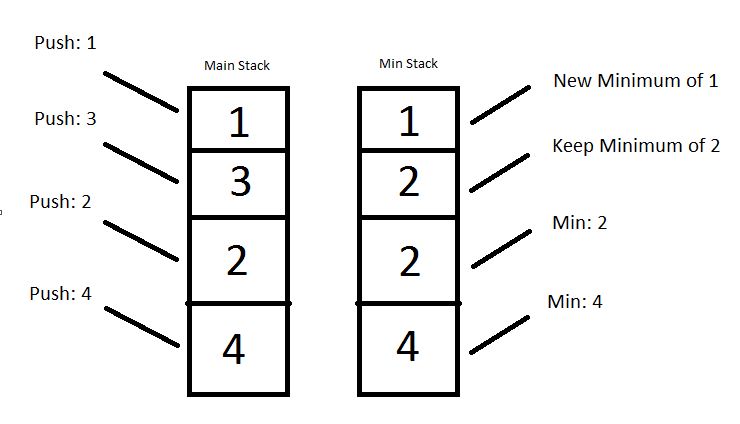
\includegraphics[width=\linewidth]{Question2new.png}
\\
\\
\end{solution}

\begin{exercise}{(3)} 
Prove by induction the formula:  F$_{n}$ = $\frac{1}{\sqrt{5}}((\frac{1 + \sqrt{5}}{2})^N - (\frac{1 - \sqrt{5}}{2})^N)$
\end{exercise}

\begin{bas}
The basis $F_{0} = 0$, and $F_{1} = 1$ is shown below to be true. So we can assume it is true for all values of N that are equal to or greater than 0. Furthermore, we can derive certain definitions below from this information.
\begin{align*}
F_{0} & =\frac{1}{\sqrt{5}}((\frac{1 + \sqrt{5}}{2})^0 - (\frac{1 - \sqrt{5}}{2})^0)\\
& =\frac{1}{\sqrt{5}}(1 - 1)\\
& = \frac{1}{\sqrt{5}}(0)\\
& = 0\\
\\
F_{1} & =\frac{1}{\sqrt{5}}((\frac{1 + \sqrt{5}}{2})^1 - (\frac{1 - \sqrt{5}}{2})^1)\\
& =\frac{1}{\sqrt{5}}((1.61) - (-.61))\\
& = \frac{1.61}{\sqrt{5}}+\frac{.61}{\sqrt{5}}\\
& = .72 + .28\\
& = 1
\\
F_{2} & =\frac{1}{\sqrt{5}}((\frac{1 + \sqrt{5}}{2})^2 - (\frac{1 - \sqrt{5}}{2})^2)\\
& =\frac{1}{\sqrt{5}}((2.61) - (.381))\\
& = \frac{2.61}{\sqrt{5}}-\frac{.381}{\sqrt{5}}\\
& = 1.17 - .17 \\
& = 1
\end{align*}
\end{bas}

\begin{defn*}
\begin{align}
F_{N} & = F_{N-1} + F_{N-2} && (\text{Derived from $F_{2} = F_{1} + F_{0}$})\\
X_{1} & = (\frac{1 + \sqrt{5}}{2})\\
X_{2} & = (\frac{1 - \sqrt{5}}{2})\\
X^{N} & = X^{N-1} + X^{N-2} && (\text{Derived from quadratic relationship})
\end{align}
\end{defn*}

\begin{solution}{(3)}
Solving for F$_{n}$ = $\frac{1}{\sqrt{5}}((\frac{1 + \sqrt{5}}{2})^N - (\frac{1 - \sqrt{5}}{2})^N)$. We can solve for $F_{N} = F_{N-1} + F_{N-2}$ by the inductive hypothesis:
\begin{align*}
F_{N} & =\frac{1}{\sqrt{5}}((\frac{1 + \sqrt{5}}{2})^{N-1} - (\frac{1 - \sqrt{5}}{2})^{N-1} + \frac{1}{\sqrt{5}}((\frac{1 + \sqrt{5}}{2})^{N-2} - (\frac{1 - \sqrt{5}}{2}))^{N-2} \\
& =\frac{1}{\sqrt{5}}((X_{1})^{N-1} - (X_{2})^{N-2} + (X_{1})^{N-1} - (X_{2})^{N-2} && (\text{Insert from above definition from (4)})\\
& = \frac{1}{\sqrt{5}}(X_{1}^N + X_{2}^N) && (\text{Insert into $F_N$ from definition (1)})\\
F_{N} & = \frac{1}{\sqrt{5}}(X_{1}^N + X_{2}^N) && (\text{expand right side to equal $F_{N}$})\\
\end{align*}
\end{solution}

\begin{exercise}{(4)} %You can use theorem, proposition, exercise, or reflection here.  Modify x.yz to be whatever number you are proving
Solve the following recurrence, which has T(0) = T(1) = 1. A Big-Oh answer will suffice.
\end{exercise}

\begin{solution}{(4)}
The average successful search is done in $O(\log n)$ time.
\begin{proof}
\begin{align*}
T(N) & = T(\frac{N}{2}) + 1\\
& = T(\frac{N}{4}) + 1 + 1\\
& = T(\frac{N}{8}) + 1 + 1 + 1\\
& = T(\frac{N}{16}) + 1 + 1 + 1 + 1\\
& = T(\frac{N}{2^k}) + x + x + ... + x && (\text{Insert n = $2^k$, and $k = \log n$})\\
& = k * x + T(1)\\
T(N) & = x*\log n\\
T(N) & = 1*\log n\\
 & O(\log n)\\
\end{align*}
\end{proof}
\end{solution}



\begin{exercise}{(5)} %You can use theorem, proposition, exercise, or reflection here.  Modify x.yz to be whatever number you are proving
Solve the following recurrence, which in all cases have T(0) = T(1) = 1. A Big-Oh answer will suffice
\end{exercise}

\begin{solution}{(5)}
The average successful search is done in $O(\log^{2} n)$ time.
\begin{proof}
\begin{align*}
T(N)  & = T(\frac{N}{2}) + \log n\\
& = \log n + \log{\frac{n}{2}}+ \log{\frac{n}{4}} + ...+ \log 1 + 1\\
& = (\log n - 0) + (\log n - 1) + ... + (\log n - \log n) + 1\\
& = (\log n *  \log n) - \frac{\log n * (\log n + 1)}{2} + 1\\
& = \frac{\log n * (\log n)}{2} - \frac{\log n}{2} + 1\\
& O(\log^2 n)
\end{align*}
\end{proof}
\end{solution}



% --------------------------------------------------------------
%     You don't have to mess with anything below this line.
% --------------------------------------------------------------
 
\end{document}